% TU Delft Beamer template
% Author: Maarten Abbink
% Delft University of Technology
% March 2014
% Version 2.0
% Based on original version 1.0 of Carl Schneider
\documentclass{beamer}
\usepackage[english]{babel}
\usepackage{calc}
\usepackage[absolute,overlay]{textpos}
\mode<presentation>{\usetheme{tud}}

\title[BaNaNa Talk]{Matlab Reservoir simulation toolbox MRST}
%\subtitle
%\institute[TU Delft]{Delft University of Technology}
\author{G. B. Diaz}
\date{4th April 2017}

% Insert frame before each subsection (requires 2 latex runs)
% \AtBeginSubsection[] {
% 	\begin{frame}<beamer>\frametitle{\titleSubsec}
% 		\tableofcontents[currentsection,currentsubsection]  % Generation of the Table of Contents
% 	\end{frame}
% }
% % Define the title of each inserted pre-subsection frame
% \newcommand*\titleSubsec{Next Subsection}
% % Define the title of the "Table of Contents" frame
% \newcommand*\titleTOC{Outline}

% define a symbol which can be removed if you don't need it
%\newcommand{\field}[1]{\mathbb{#1}}
%\newcommand{\Zset}{\field{Z}}

\begin{document}

{
% remove the next line if you don't want a background image
%\usebackgroundtemplate{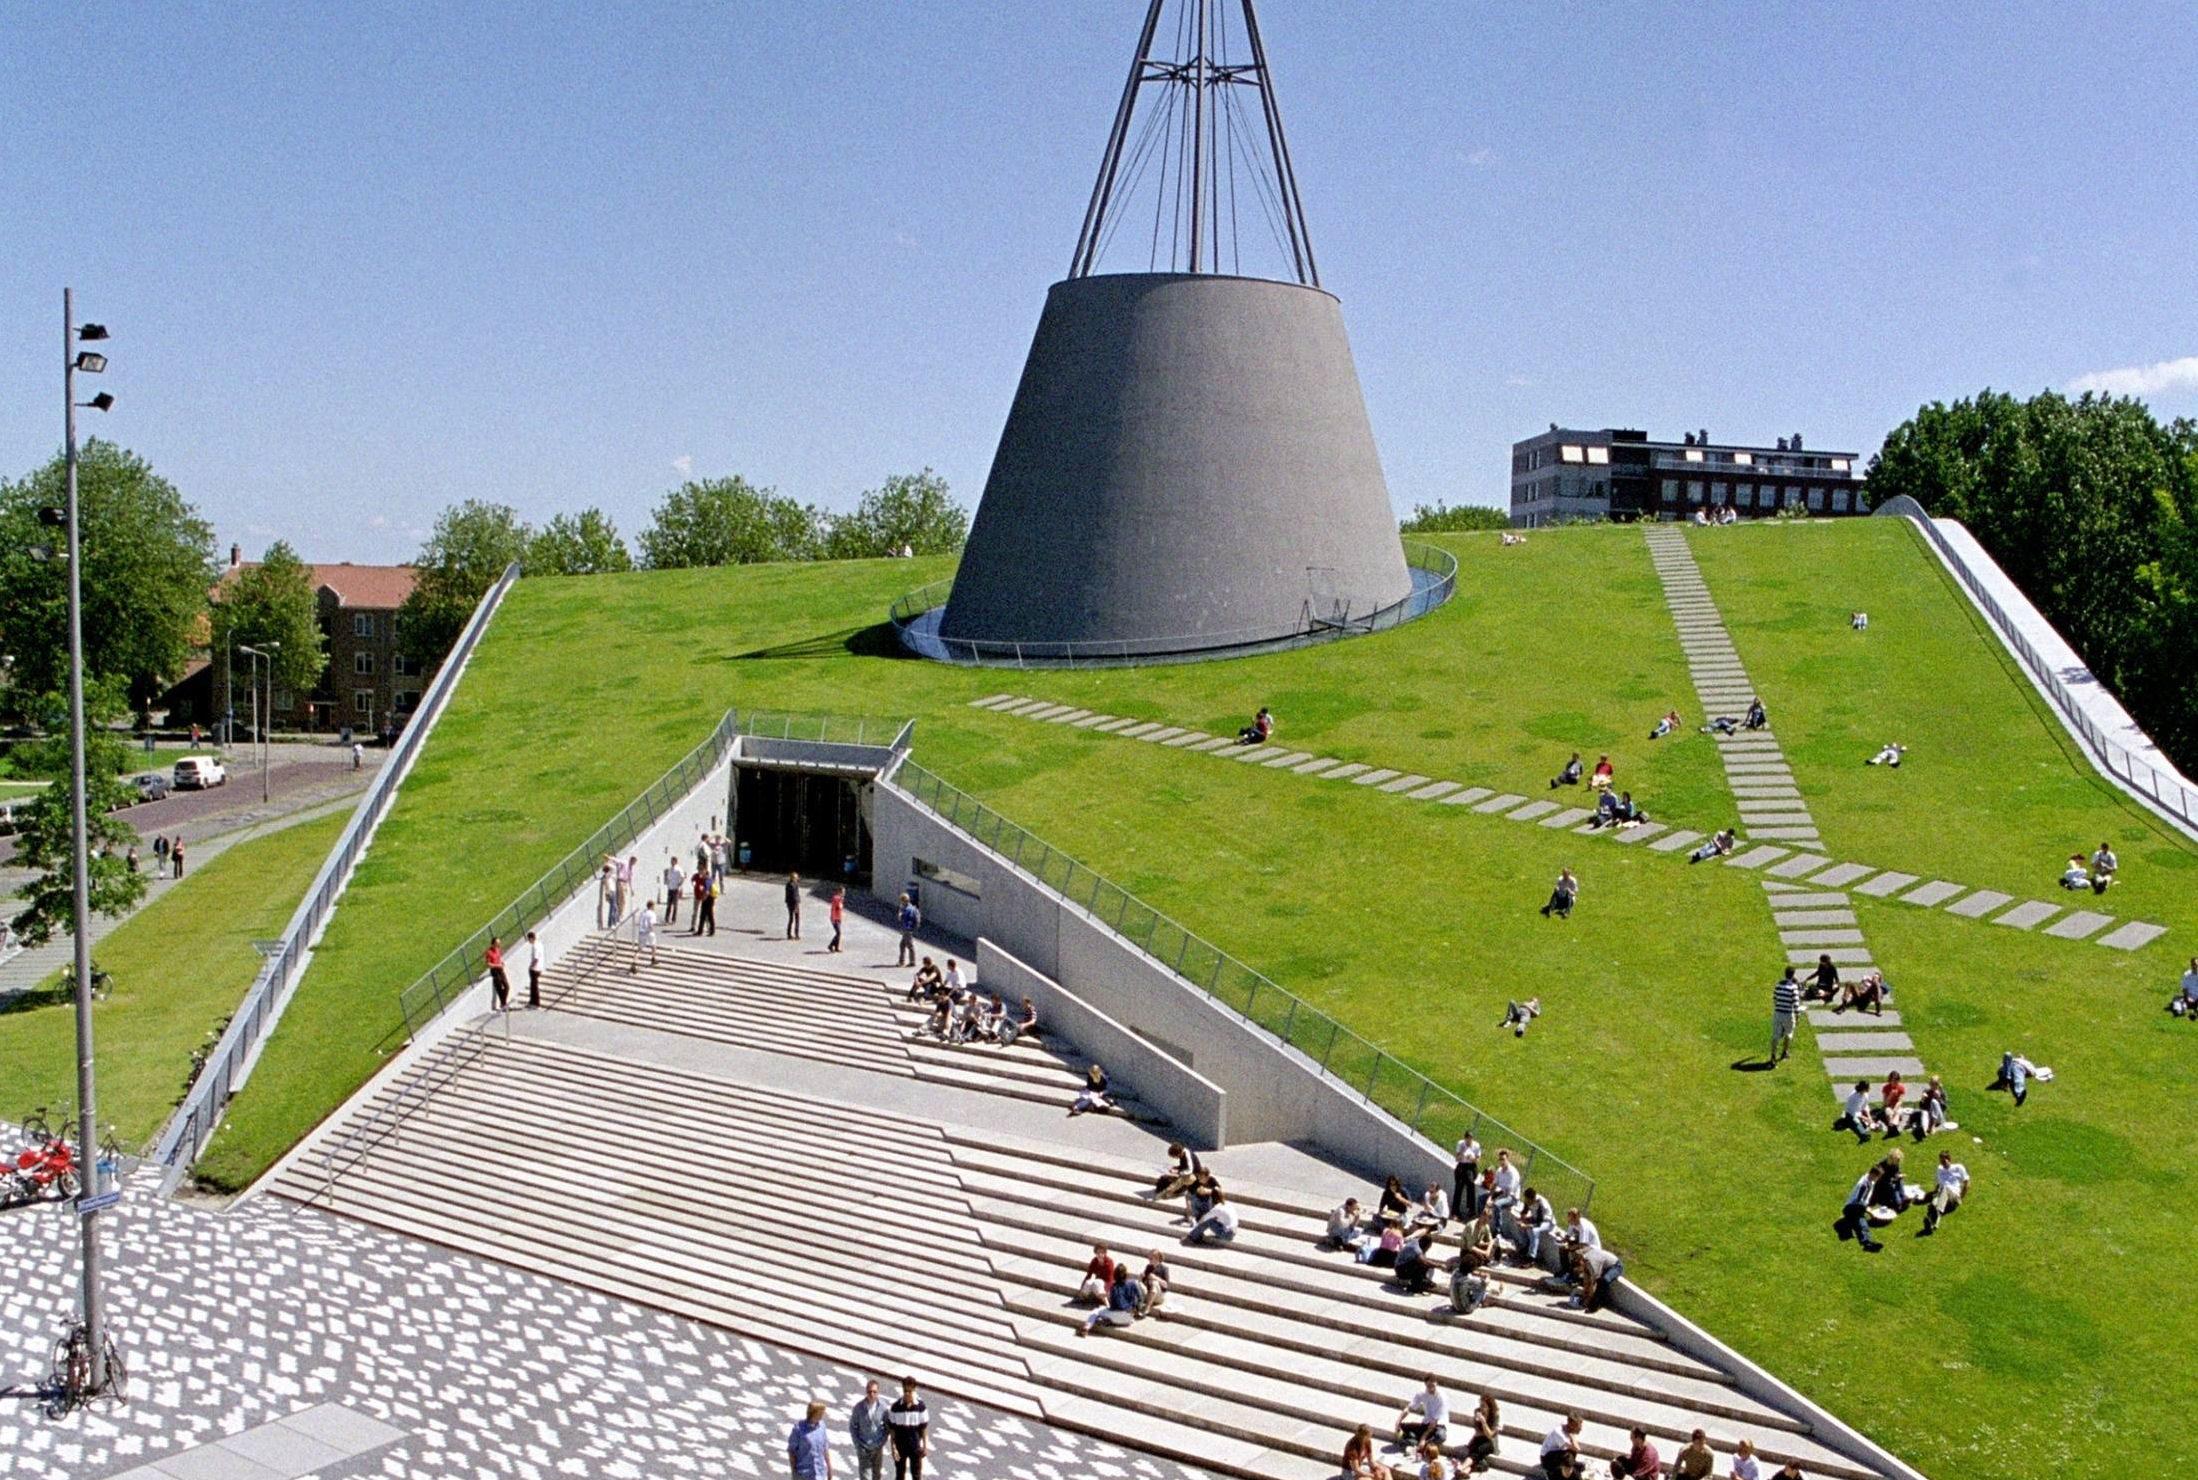
\includegraphics[width=\paperwidth,height=\paperheight]{images/background-titlepage.jpg}}%
\setbeamertemplate{footline}{\usebeamertemplate*{minimal footline}}
%\frame{\titlepage}
}





\begin{frame}[shrink=0.2]\frametitle{Matlab Reservoir simulation toolbox MRST}
	%this is too big.
	%\begin{example}
		\centering
		{
		
		\begin{minipage}{0.7\textwidth}
		G. B. Diaz Cortes\\
		

			% insert picture (pdf file)
% 			\centering{
% 			
\includegraphics[width=0.2\textwidth]{logo_tud.pdf}}
		\end{minipage}
		}
		
		\centering
		{
		\begin{figure}
		\begin{minipage}{.5\textwidth}
 \centering
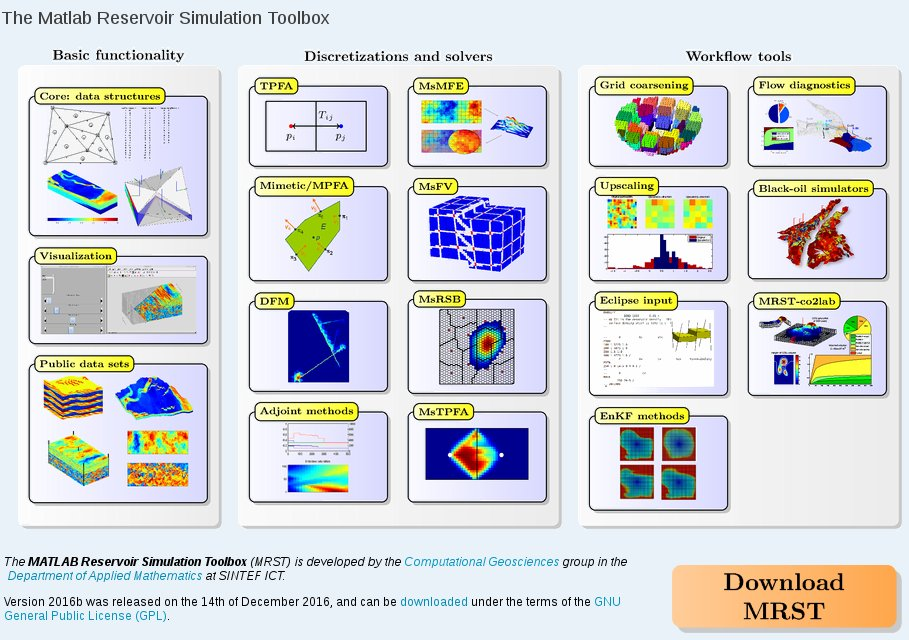
\includegraphics[width=8cm,height=8cm,keepaspectratio]
{/home/wagm/cortes/Localdisk/baNaNa/MRST/web.jpg}

\end{minipage}
{\\Website: http://www.sintef.no/projectweb/mrst/}
\end{figure}
		}
	%\end{example}
\end{frame}
\begin{frame}\frametitle{Matlab Reservoir simulation toolbox MRST}
	%this is too big.
	%\begin{example}
		\centering
		{
		
		\begin{minipage}{0.7\textwidth}
		G. B. Diaz Cortes\\
		

			% insert picture (pdf file)
% 			\centering{
% 			
\includegraphics[width=0.2\textwidth]{logo_tud.pdf}}
		\end{minipage}
		}
		
		\centering
		{
		
		\begin{minipage}{.5\textwidth}
		\begin{figure}
 \centering
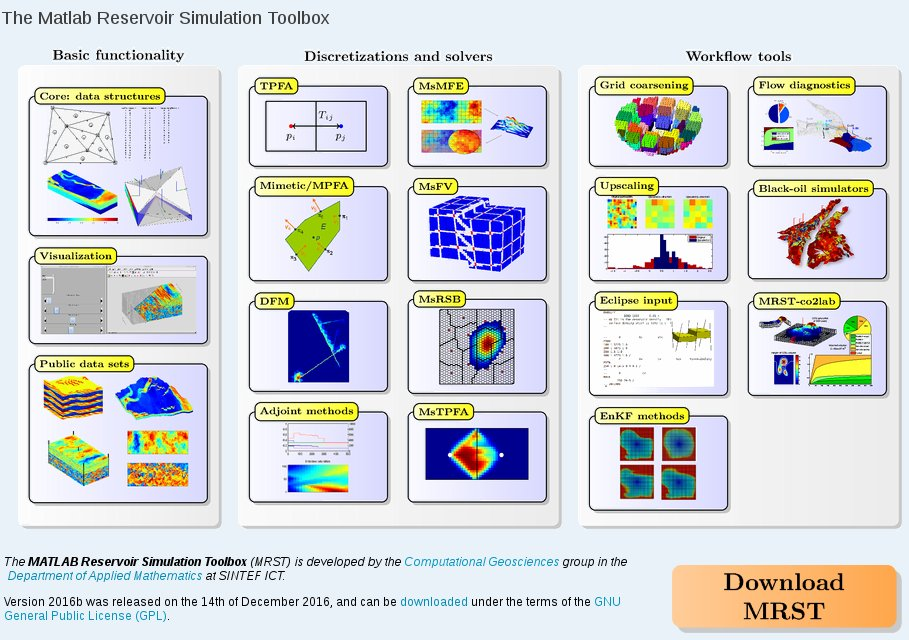
\includegraphics[width=6cm,height=6cm,keepaspectratio]
{/home/wagm/cortes/Localdisk/baNaNa/MRST/web.jpg}
\end{figure}
\end{minipage}%
		\begin{minipage}{0.5\textwidth}
		

			% insert picture (pdf file)
			\centering{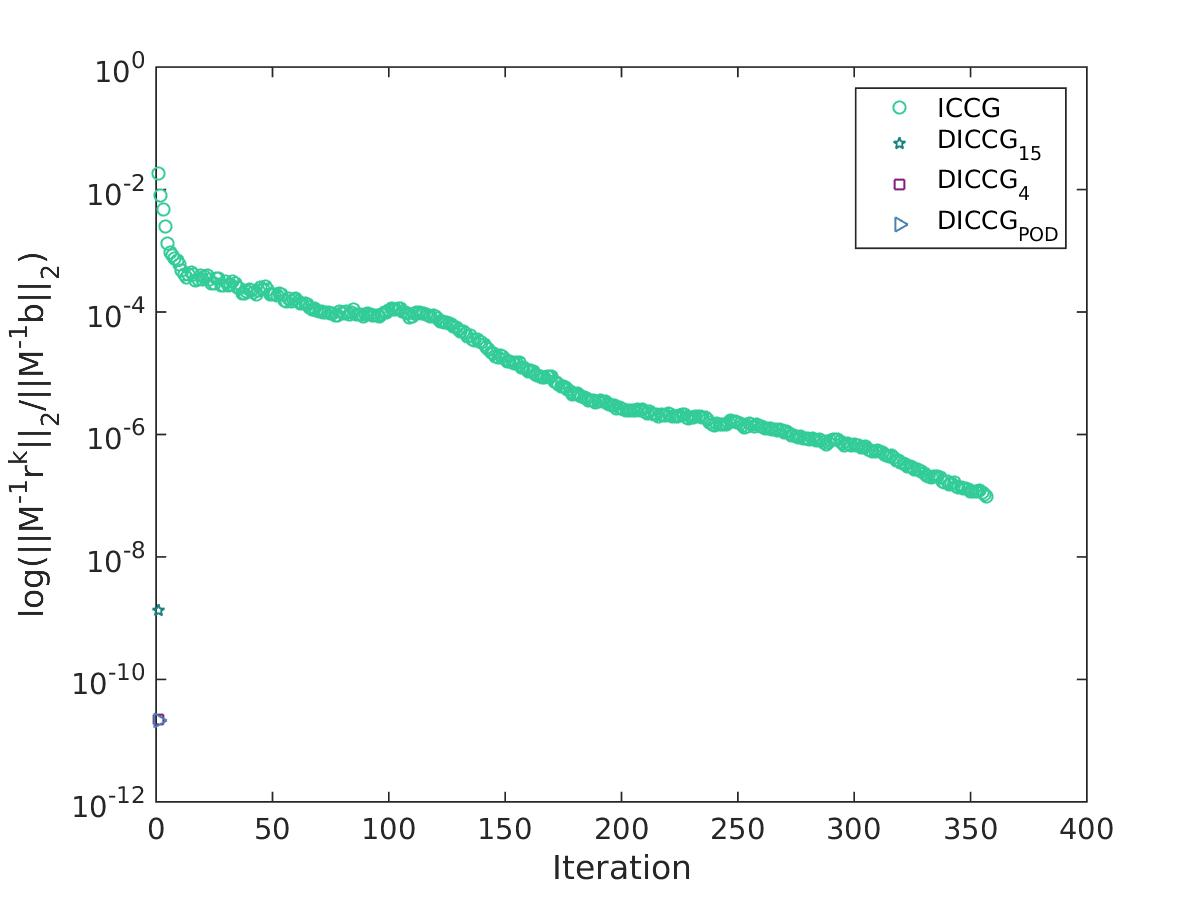
\includegraphics[width=6cm,height=6cm,keepaspectratio]
{conv_spe10c.jpg}}
		\end{minipage}
		}
	%\end{example}
\end{frame}

\end{document}
